\section{Case Studies}
\label{sec:case-studies}

\subsection{Case 1: The Poisson Equation}

[TODO]

\begin{figure}
    \centering
    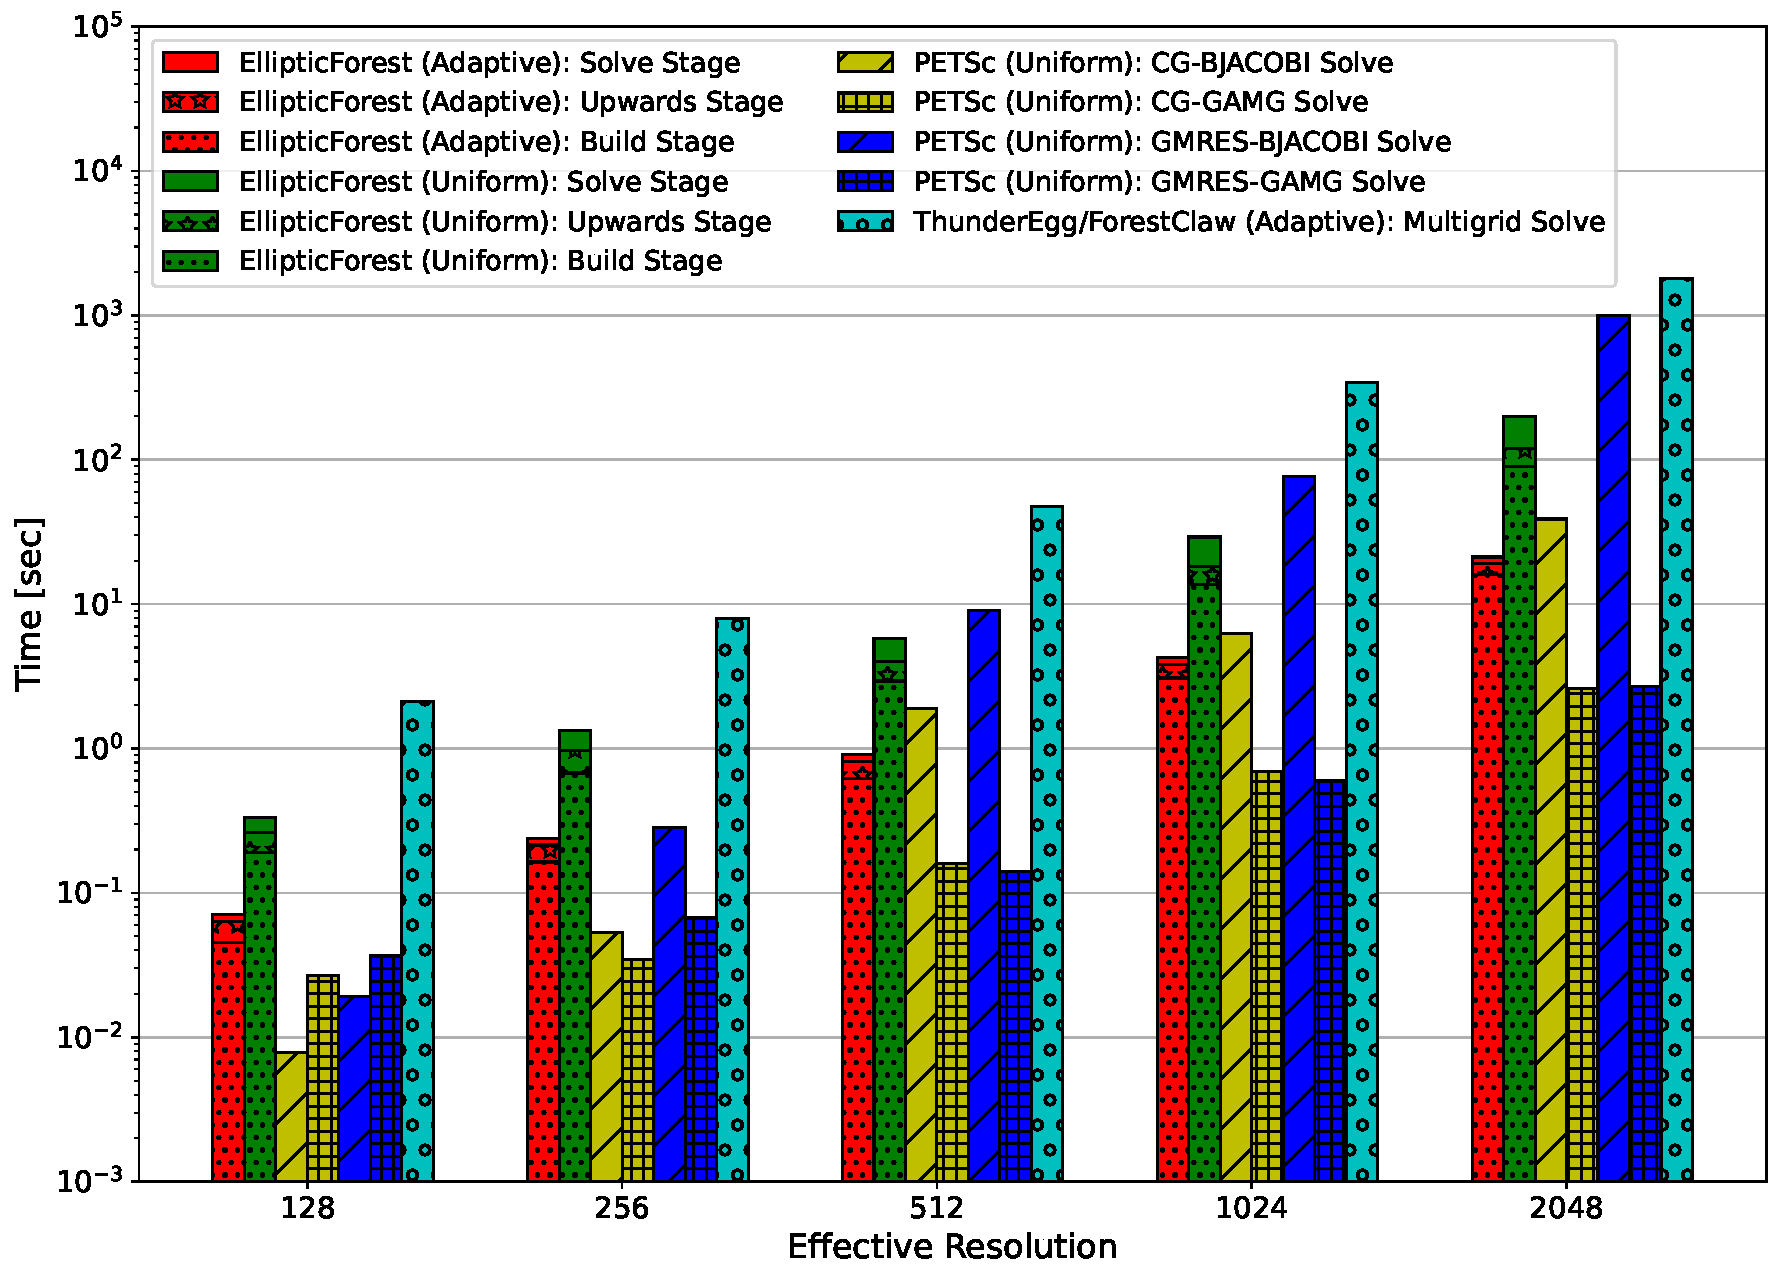
\includegraphics[width=1.0\textwidth, clip=true, trim={60 20 100 60}]{figures/case01-stacked-bar-plot-comparisons-no-title.pdf}
    \caption{[TODO]}
    \label{fig:case01-stacked-bar-plot}
\end{figure}

\begin{figure}
    \centering
    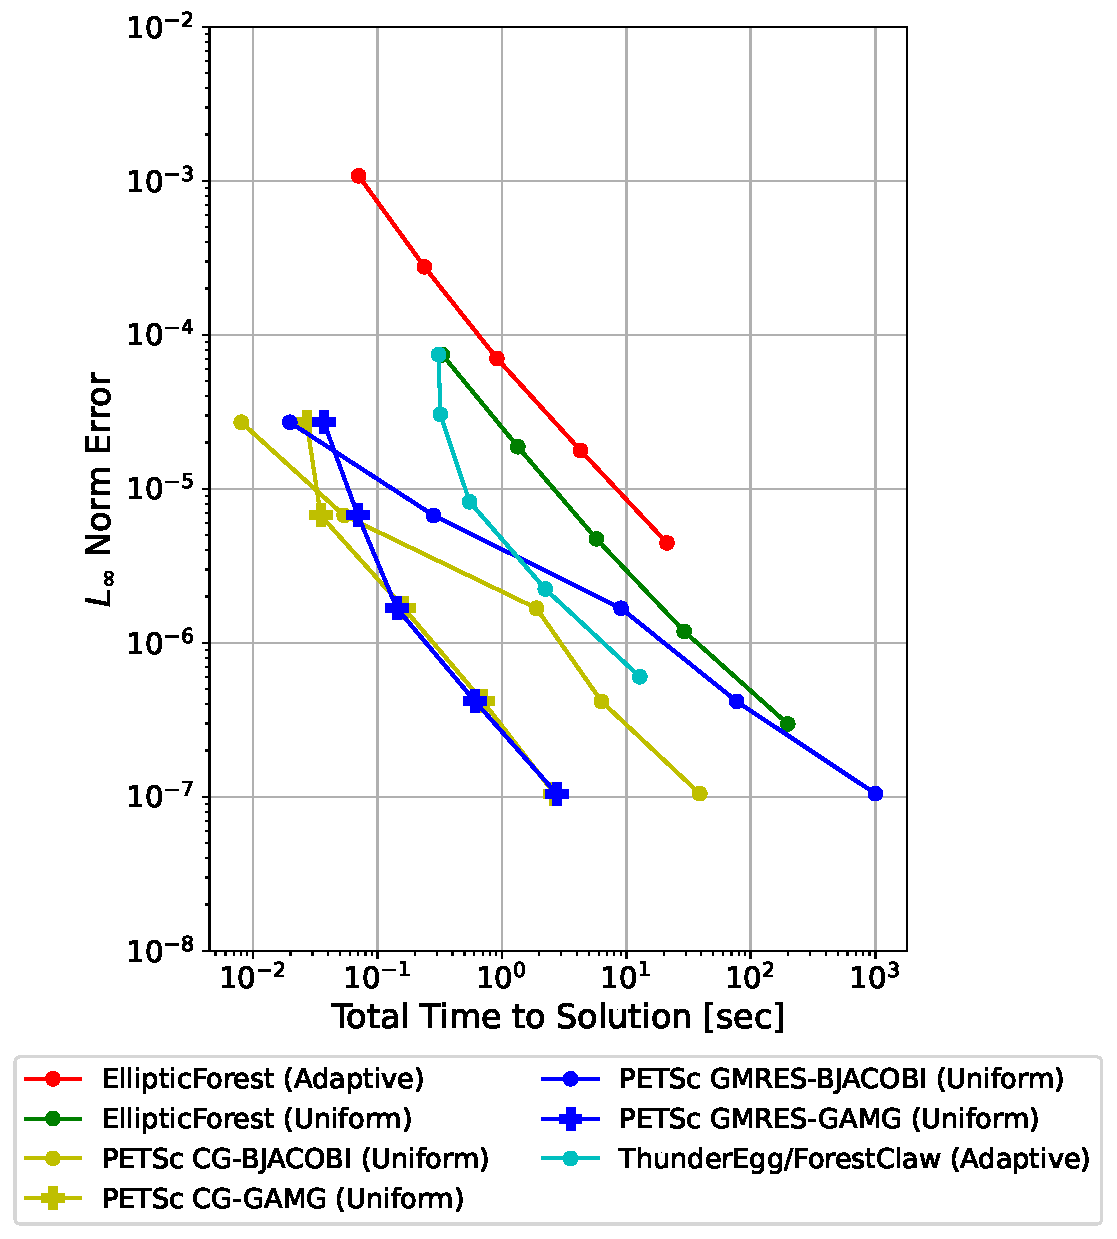
\includegraphics[width=1.0\textwidth, clip=true, trim={40 20 80 50}]{figures/case01-work-precision-plots-no-title.pdf}
    \caption{[TODO]}
    \label{fig:case01-work-precision-plot}
\end{figure}

\subsection{Case 2: Variable Coefficient Poisson Equation}

[TODO]

\begin{figure}
    \centering
    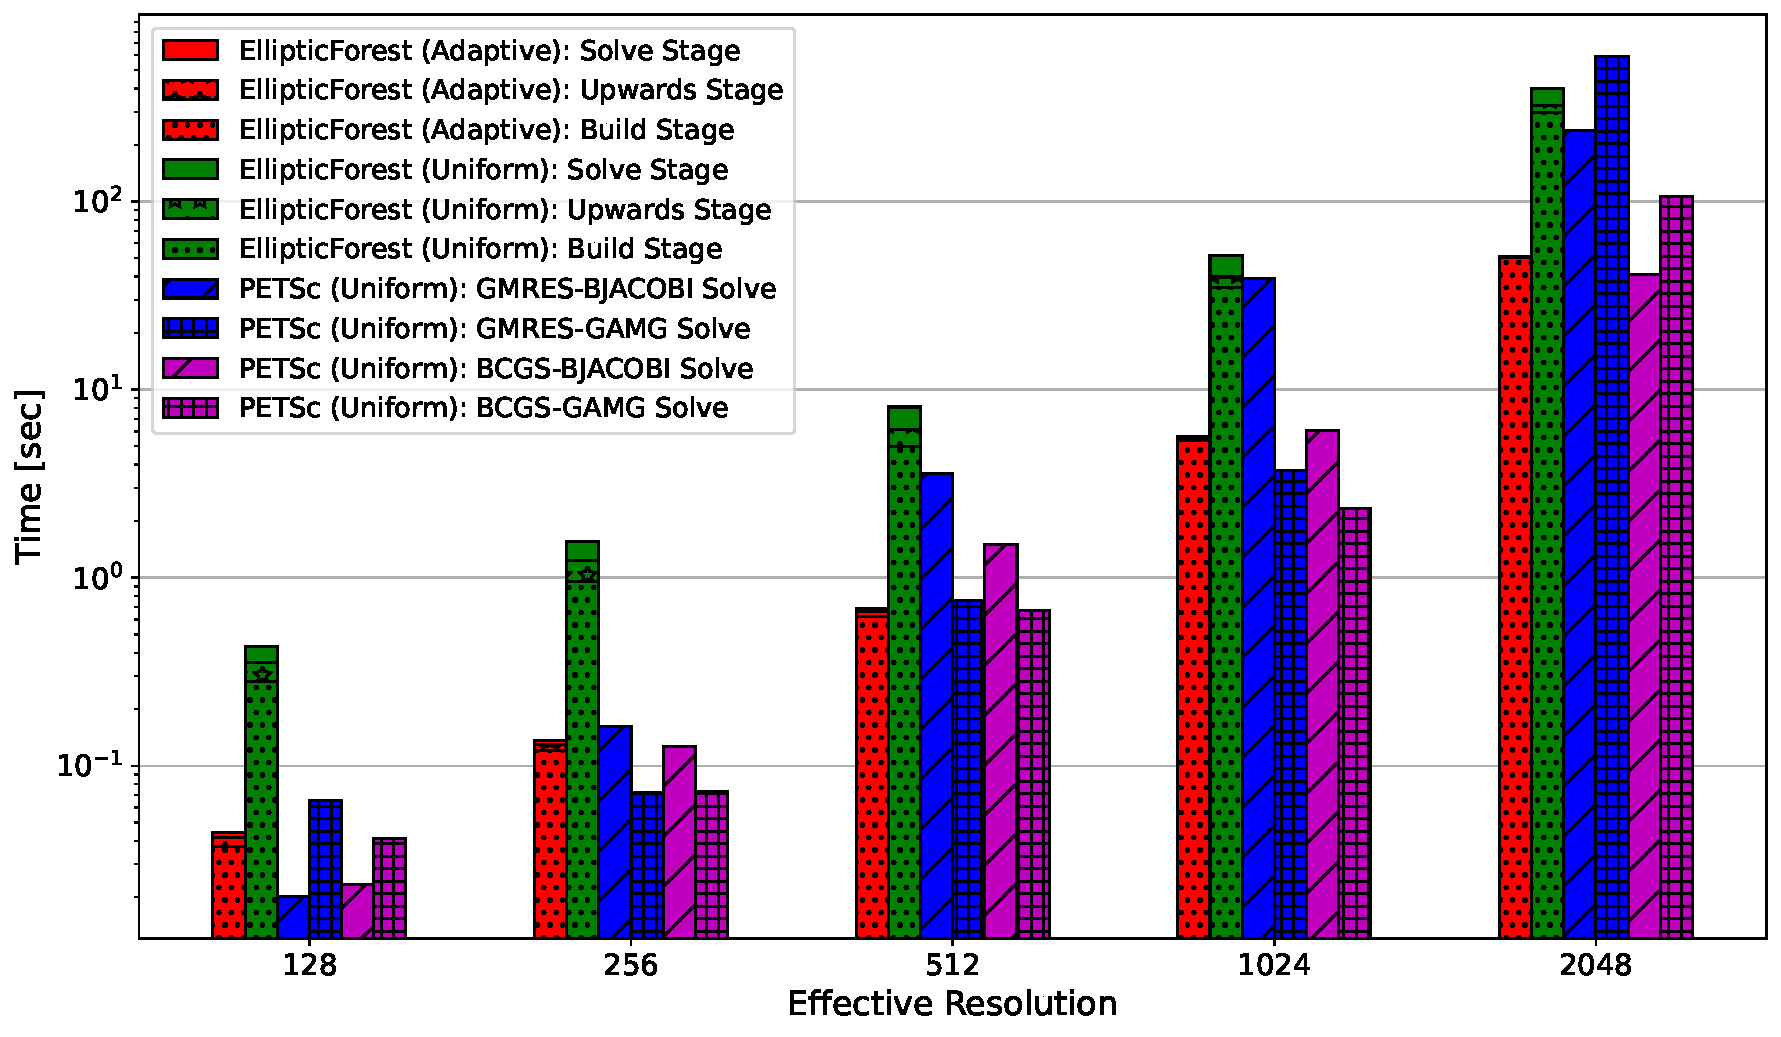
\includegraphics[width=1.0\textwidth, clip=true, trim={60 20 100 60}]{figures/case02-stacked-bar-plot-comparisons-no-title.pdf}
    \caption{[TODO]}
    \label{fig:case02-stacked-bar-plot}
\end{figure}

\begin{figure}
    \centering
    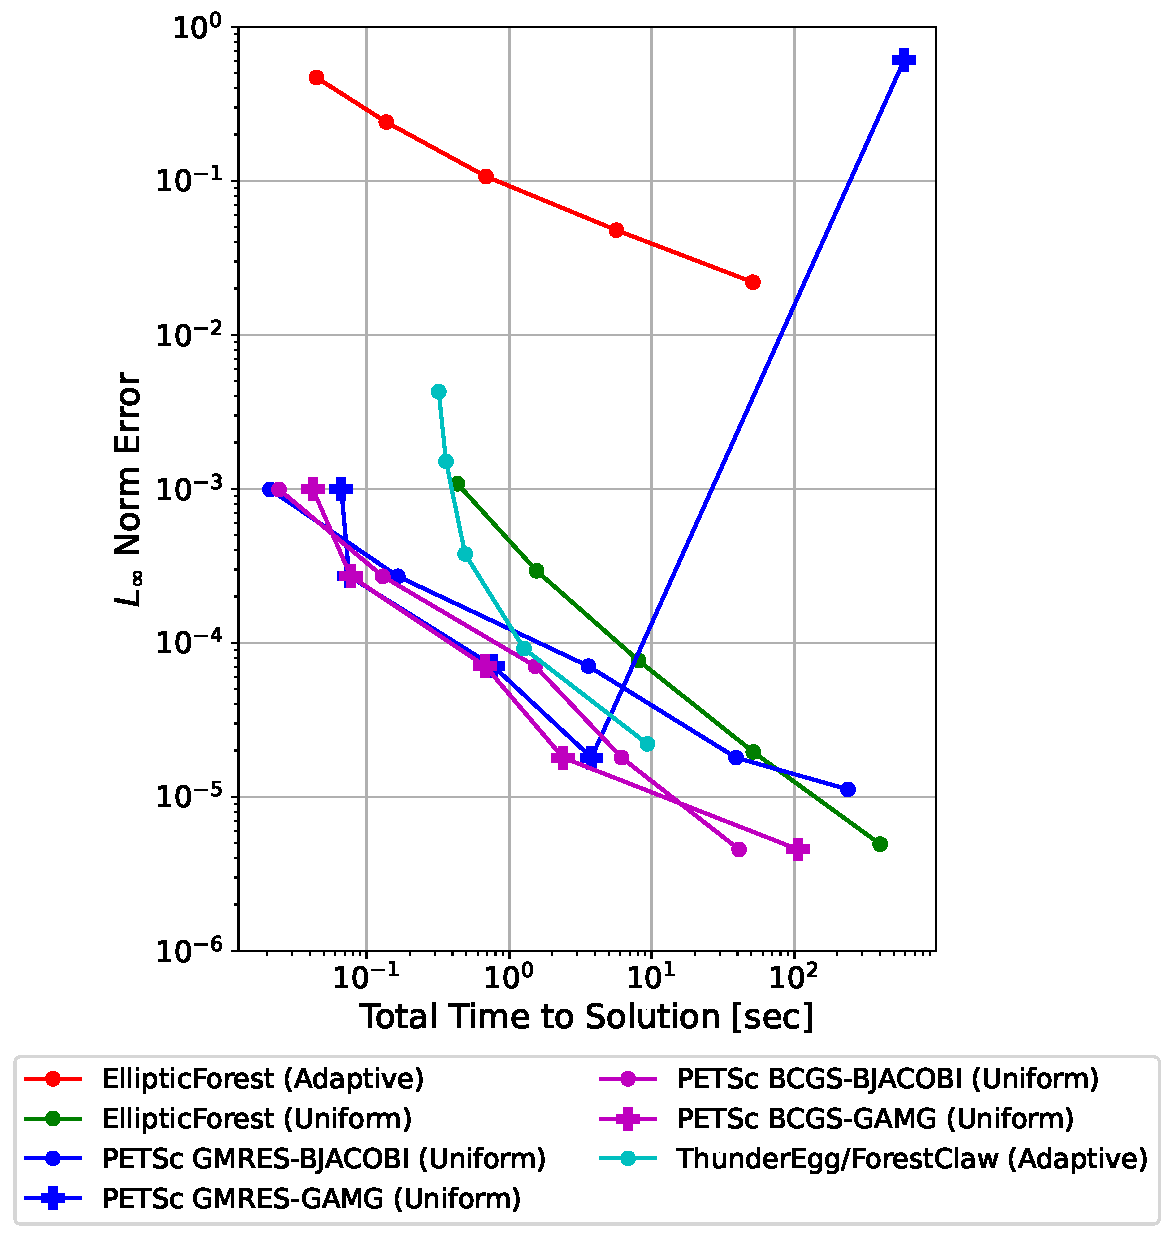
\includegraphics[width=1.0\textwidth, clip=true, trim={40 20 80 50}]{figures/case02-work-precision-plots-no-title.pdf}
    \caption{[TODO]}
    \label{fig:case02-work-precision-plot}
\end{figure}

\subsection{Case 3: Helmholtz Equation}

[TODO]

\begin{figure}
    \centering
    \begin{subfigure}[t]{0.48\textwidth}
        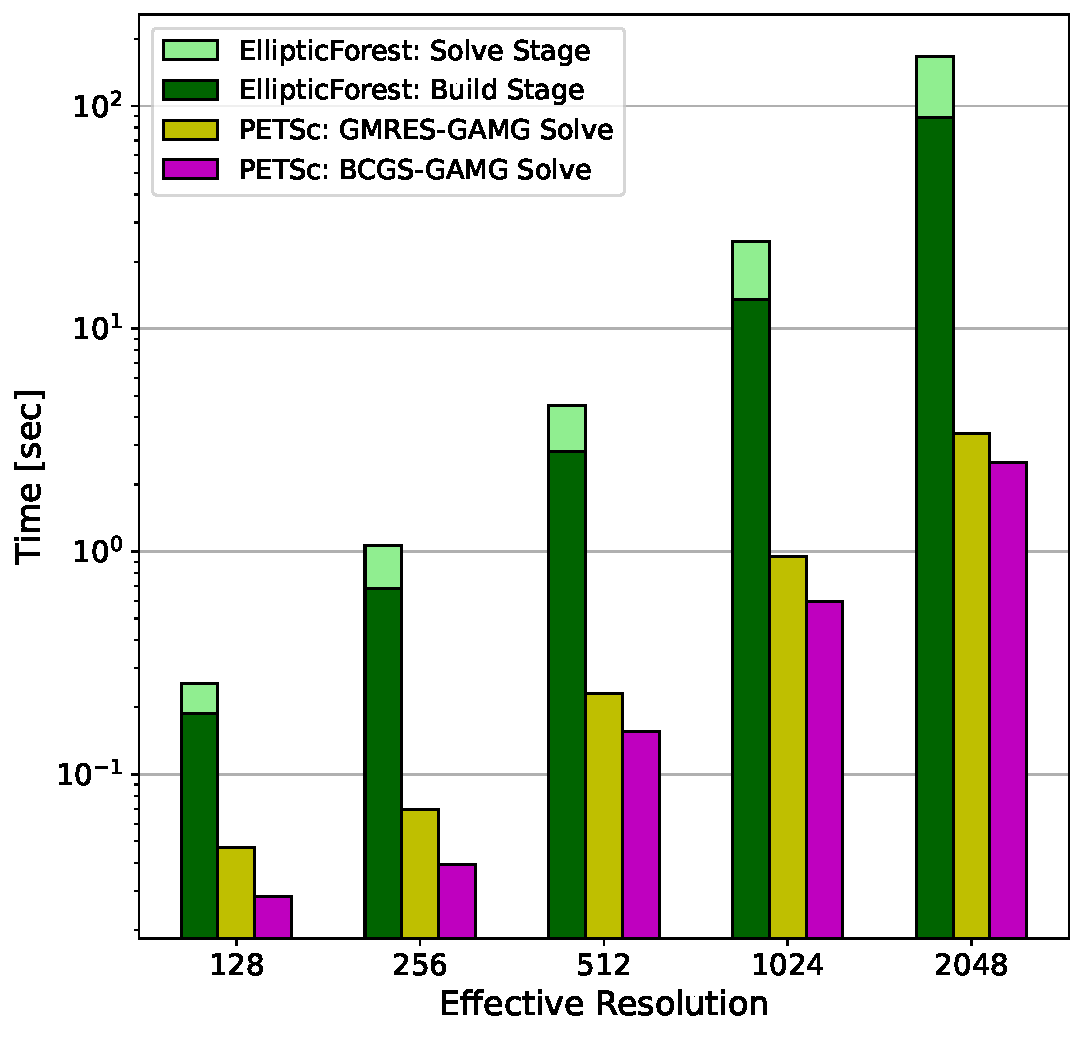
\includegraphics[width=1\textwidth, clip=true, trim={15 25 50 60}]{figures/case03-l1-stacked-bar-plot-comparisons-no-title.pdf}
        \caption{$\lambda = 1$}
    \end{subfigure}
    \begin{subfigure}[t]{0.48\textwidth}
        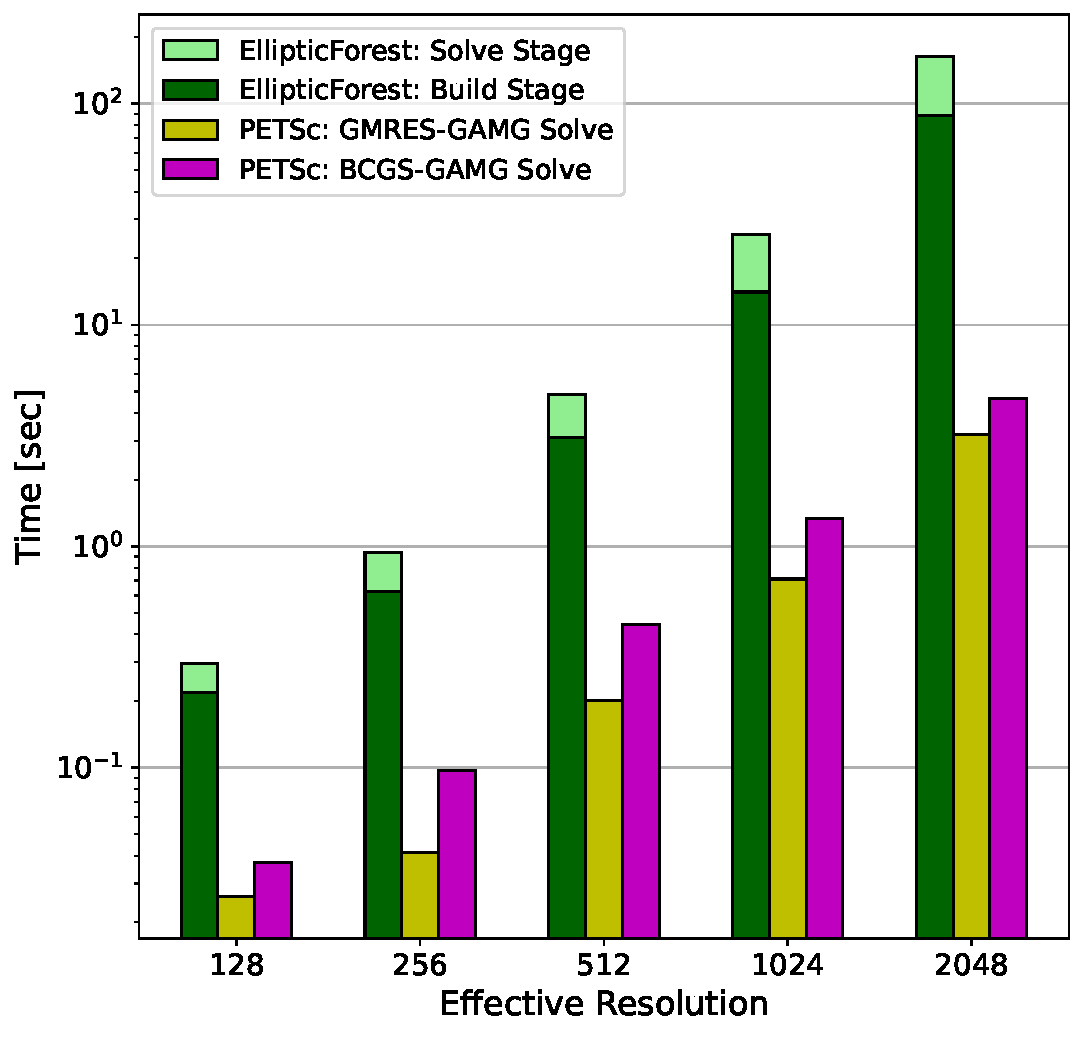
\includegraphics[width=1\textwidth, clip=true, trim={15 25 50 60}]{figures/case03-l10-stacked-bar-plot-comparisons-no-title.pdf}
        \caption{$\lambda = 10$}
    \end{subfigure}
    \begin{subfigure}[t]{0.48\textwidth}
        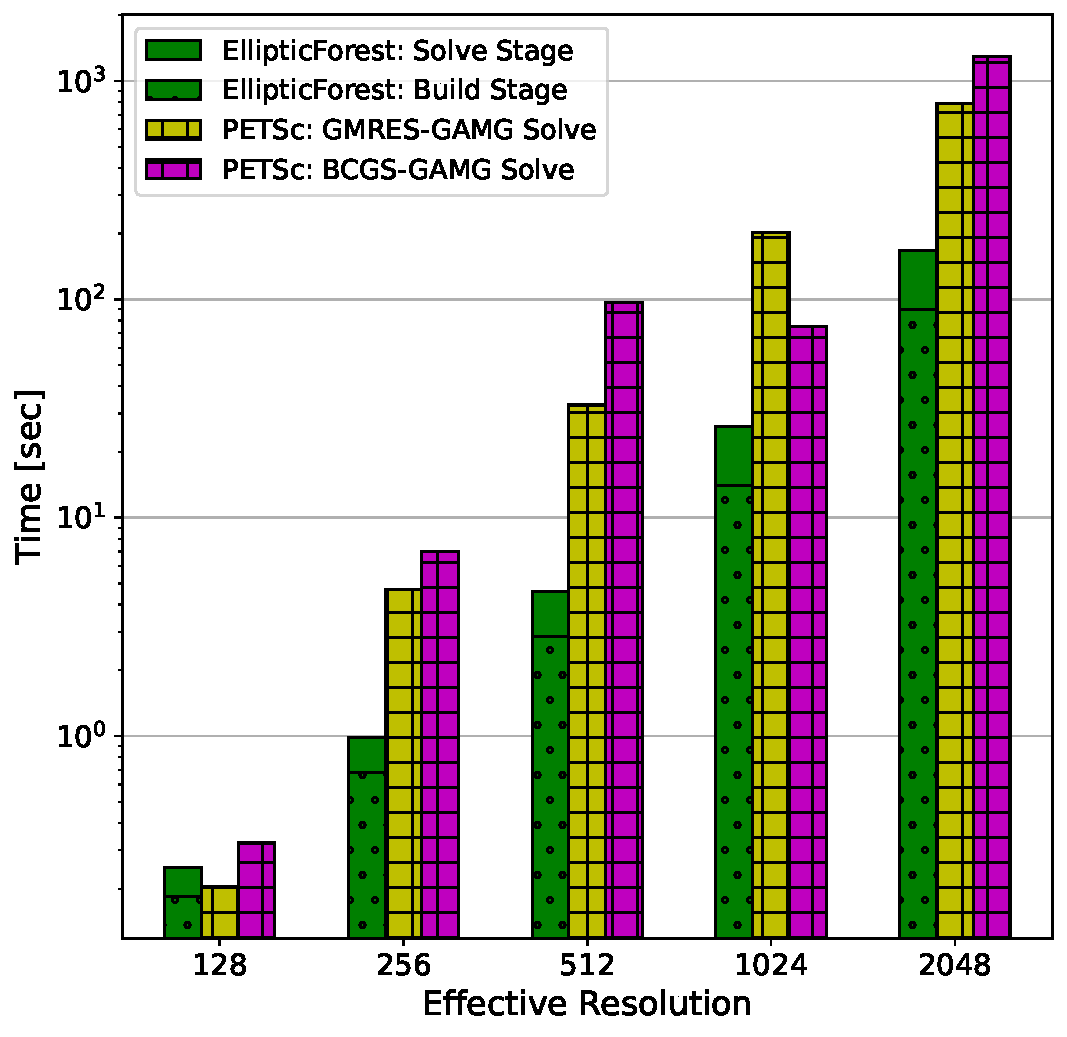
\includegraphics[width=1\textwidth, clip=true, trim={15 25 50 60}]{figures/case03-l100-stacked-bar-plot-comparisons-no-title.pdf}
        \caption{$\lambda = 100$}
    \end{subfigure}
    \begin{subfigure}[t]{0.48\textwidth}
        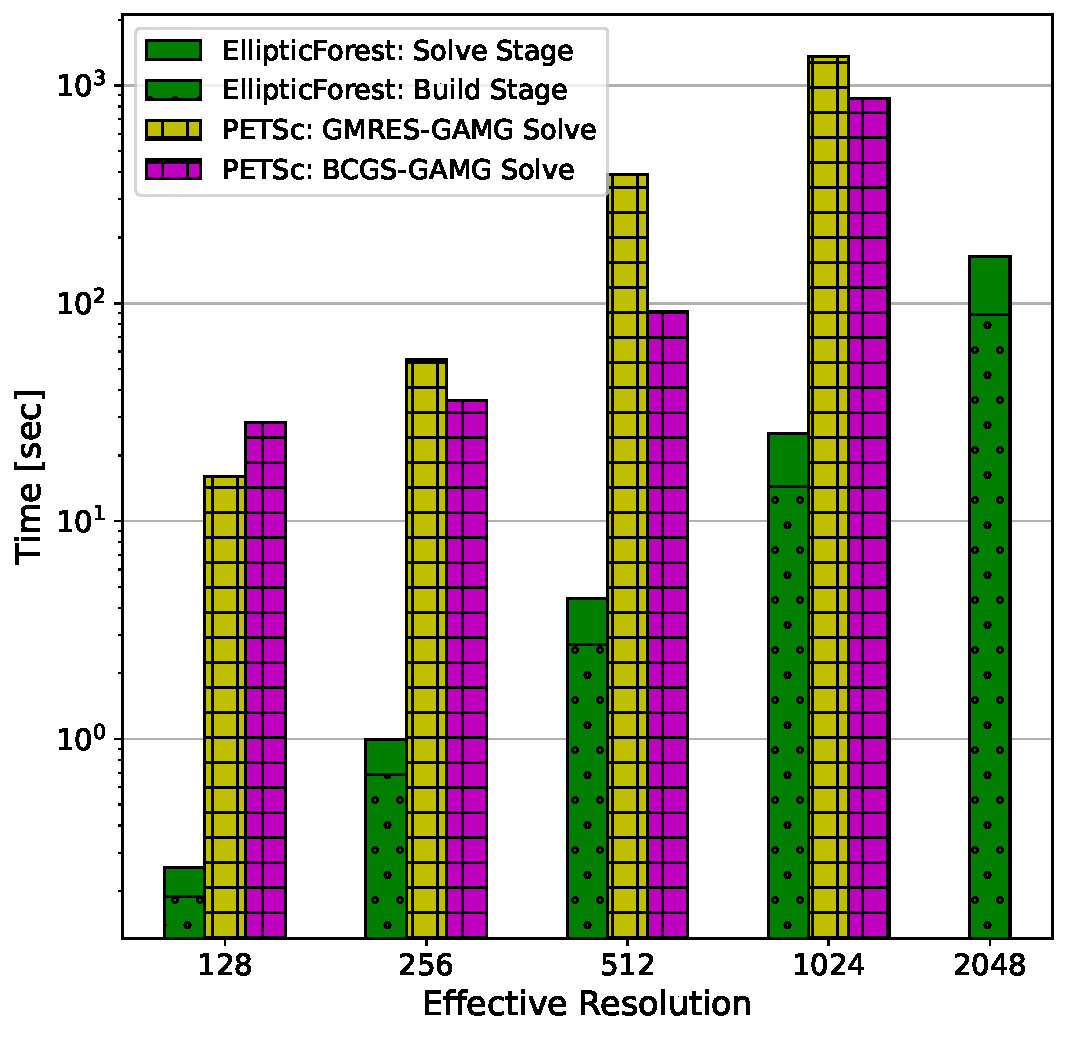
\includegraphics[width=1\textwidth, clip=true, trim={15 25 50 60}]{figures/case03-l1000-stacked-bar-plot-comparisons-no-title.pdf}
        \caption{$\lambda = 1000$}
    \end{subfigure}
    \caption{[TODO]}
    \label{fig:case03-stacked-bar-plot}
\end{figure}

\begin{figure}
    \centering
    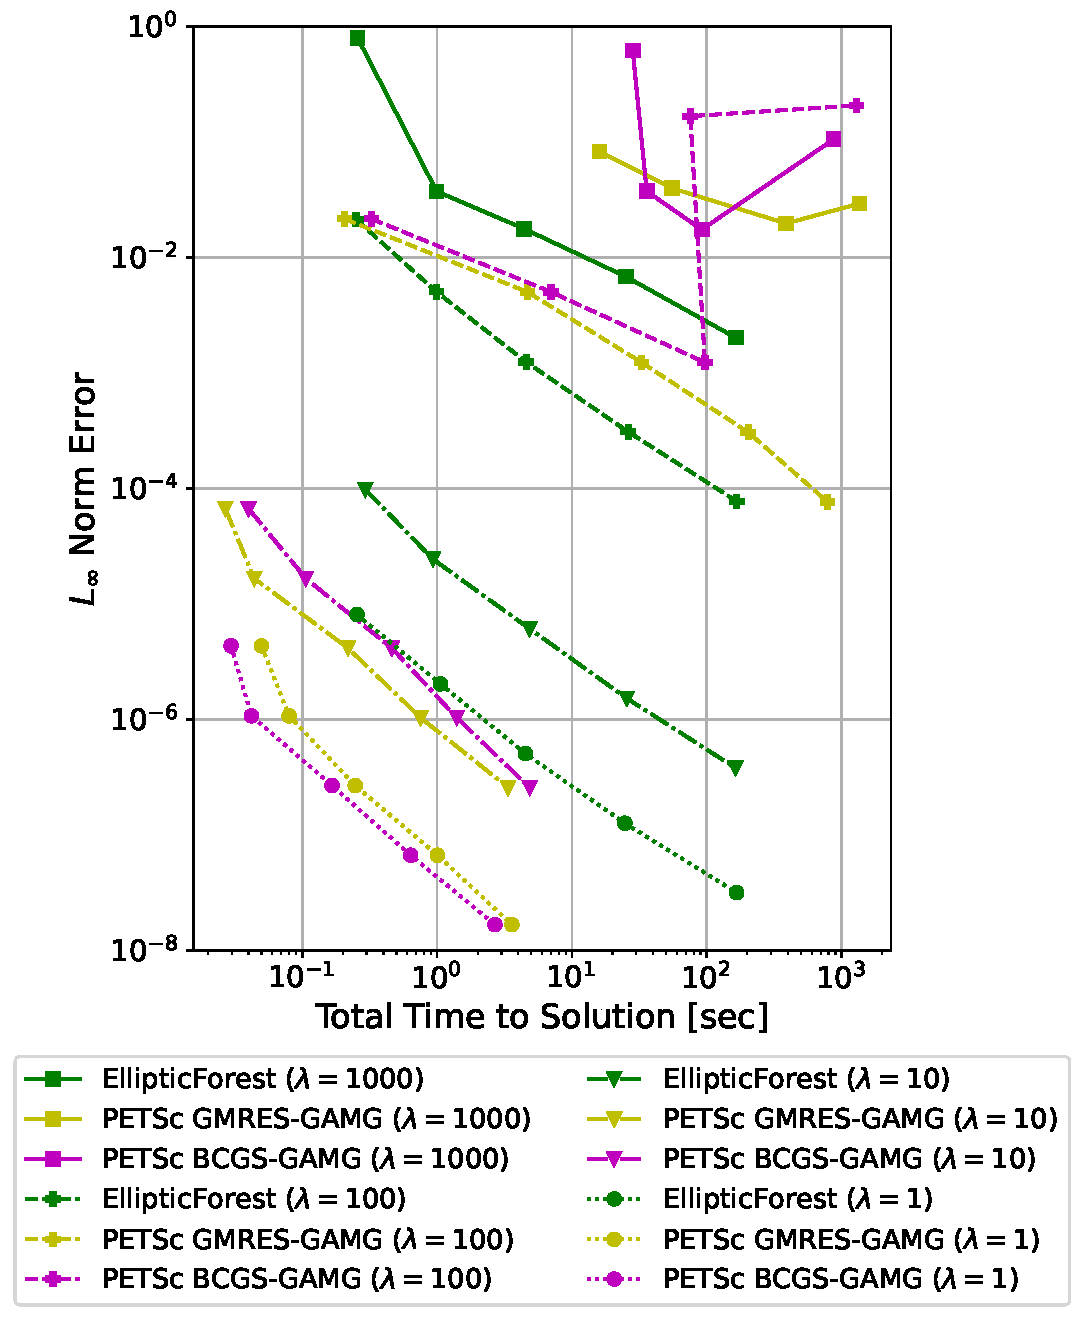
\includegraphics[width=1.0\textwidth, clip=true, trim={0 0 0 0}]{figures/case03-work-precision-plots-no-title.pdf}
    \caption{[TODO]}
    \label{fig:case03-work-precision-plot}
\end{figure}